%!TEX TS-program = xelatex
\documentclass[aspectratio=169]{beamer}
\usetheme{hust}

\usepackage{qrcode}
\usepackage{graphicx}
\usepackage{xcolor}
\usepackage[absolute,overlay]{textpos}
\usepackage{tikz}
\usepackage{calc}
\usepackage{polyglossia}
\setmainlanguage{english}
\usepackage{amsthm,amsmath,amssymb}
\newtheorem{thm}{Theory}
\newtheorem{defn}{Definition}
\usepackage{subcaption}
\usepackage{dutchcal}
\usepackage{url}

%%%%%%%%%%%%%%%%%%%%%%%%%%%%%%%%%%%%%%%%%%%%%%%%%%%%%%%%%%%%%%%%%%%%%%
% LaTeX Overlay Generator - Annotated Figures v0.0.1
% Created with http://ff.cx/latex-overlay-generator/
%%%%%%%%%%%%%%%%%%%%%%%%%%%%%%%%%%%%%%%%%%%%%%%%%%%%%%%%%%%%%%%%%%%%%%
%\annotatedFigureBoxCustom{bottom-left}{top-right}{label}{label-position}{box-color}{label-color}{border-color}{text-color}
\newcommand*\annotatedFigureBoxCustom[8]{\draw[#5,thick,rounded corners] (#1) rectangle (#2);\node at (#4) [fill=#6,thick,shape=circle,draw=#7,inner sep=2pt,font=\sffamily,text=#8] {\textbf{#3}};}
%\annotatedFigureBox{bottom-left}{top-right}{label}{label-position}
\newcommand*\annotatedFigureBox[4]{\annotatedFigureBoxCustom{#1}{#2}{#3}{#4}{gray}{gray}{black}{black}}
\newcommand*\annotatedFigureText[4]{\node[draw=none, anchor=south west, text=#2, inner sep=0, text width=#3\linewidth,font=\sffamily] at (#1){#4};}
\newenvironment {annotatedFigure}[1]{\centering\begin{tikzpicture}
\node[anchor=south west,inner sep=0] (image) at (0,0) { #1};\begin{scope}[x={(image.south east)},y={(image.north west)}]}{\end{scope}\end{tikzpicture}}
%%%%%%%%%%%%%%%%%%%%%%%%%%%%%%%%%%%%%%%%%%%%%%%%%%%%%%%%%%%%%%%%%%%%%%

\DeclareGraphicsExtensions{.eps, .pdf, .png, .jpeg, .jpg}
\graphicspath{{figures/}{diagrams/}}

% \setbeameroption{show notes} % show notes and slides
\setbeameroption{show notes on second screen=right} % show slides with notes on the bottom
% \setbeameroption{hide notes} % Only slides
% \setbeameroption{show only notes} % show only notes
% \addtobeamertemplate{note page}{}{\thispdfpagelabel{notes:\insertframenumber}}
\setbeamertemplate{note page}[plain]
\setbeamertemplate{theorems}[numbered]
\setbeamertemplate{caption}[numbered]

\newcommand{\Image}[1]{%
    \sbox0{\includegraphics[height=0.65\paperheight]{#1}}%
    \ifdim\wd0 < \textwidth
    \includegraphics[height=0.65\paperheight]{#1}%
  \else
  \includegraphics[width=\textwidth]{#1}%
  \fi%
}

\AtBeginSubsection[]
{
  \begin{frame}{Table of contents}
    \tableofcontents[currentsection, subsectionstyle=show/shaded/hide, subsubsectionstyle=show/show/show/hide]
  \end{frame}
}

% NOTE: Important! Fix text is not visible when using show notes on second screen
% https://tex.stackexchange.com/questions/232168/normal-text-is-invisible-when-using-beamer-with-notes-and-xelatex
\makeatletter 
\def\beamer@framenotesbegin{% at beginning of slide
     \usebeamercolor[fg]{normal text}
      \gdef\beamer@noteitems{}% 
      \gdef\beamer@notes{}% 
}
\makeatother

% \titlegraphic{\includegraphics[height=\logoheight]{figures/sami-v2.pdf}}
\title{Graduation Thesis}
\subtitle{Grammatical Error Correction Using Machine Learning\\Web Application (GecWeb)}

\author{Student: Ngô Văn Cảnh - 20193204 \protect\linebreak Advisor: Prof. Dương Tấn Nghĩa}

\date{February 2025}

\newcommand{\WebsiteURL}{https://gratefully-wise-redfish.ngrok-free.app}

\begin{document}
\begin{frame}[noframenumbering,Title]
  \maketitle
\end{frame}

\note{
  Greatings, everyone.

  I am Ngô Văn Cảnh from Hanoi University of Science and Technology, class ET-E4 Elitech Program.

  Today, I am going to present my graduation thesis, which is about Grammatical Error Correction using machine learning web application, or GecWeb for short.

  Under the guidance of Professor Dương Tấn Nghĩa.
}

\begin{frame}{Table of Contents}
  \tableofcontents
\end{frame}

\note{
  In today's talks, I will cover the following topics:
}

\section{Introduction}

\subsection{Motivation}

\begin{frame}{Motivation}
  \begin{figure}
    \begin{center}
      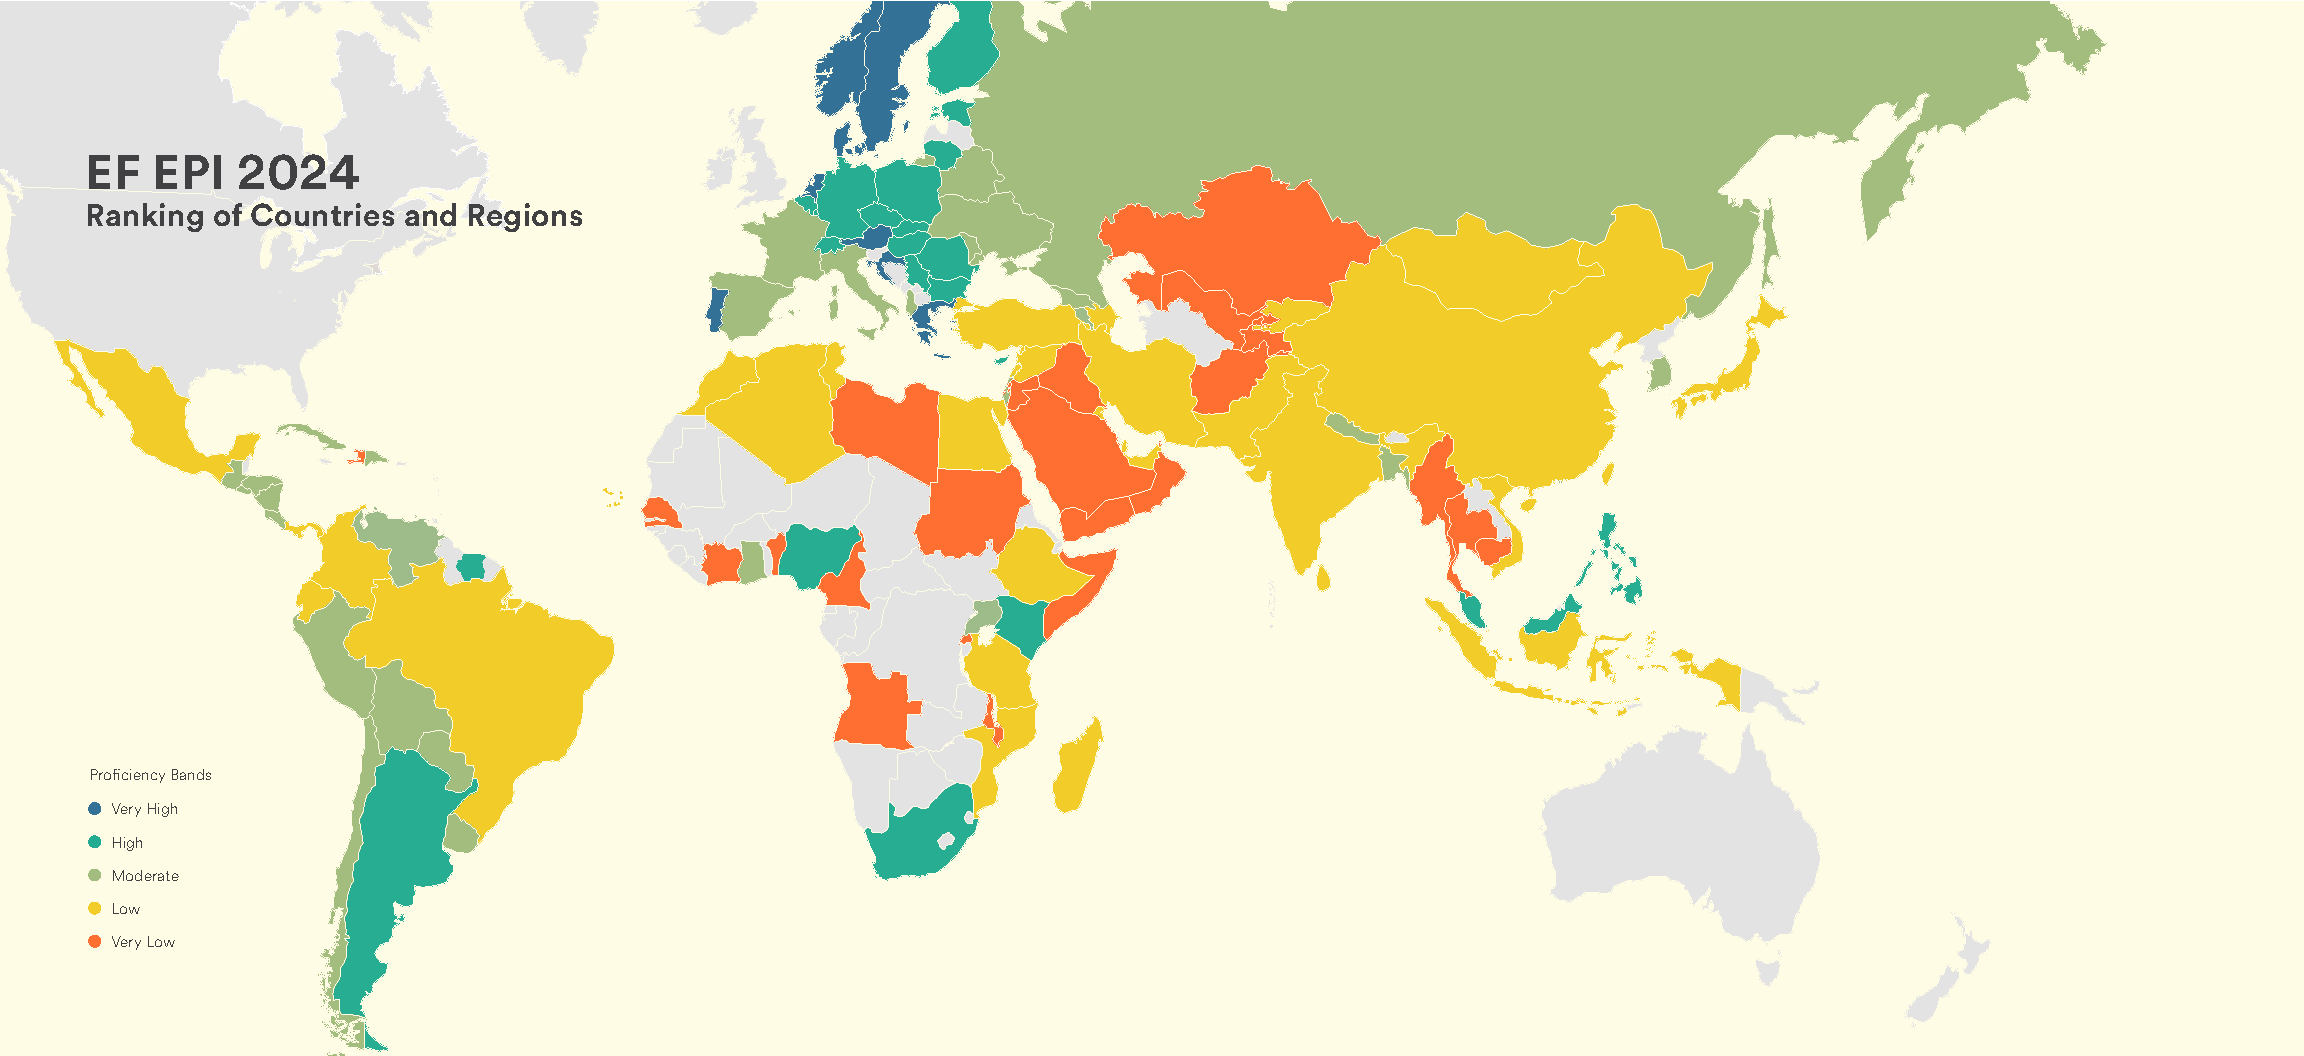
\includegraphics[width=\textwidth]{figures/ef-epi-2024-english-crop.pdf}
      \begin{textblock*}{8cm}(\paperwidth-9cm, \paperheight-2.5cm)  % (x,y) coordinates from top-left
        \textbf{\Large $> 1.4$ billion speakers}

        \textbf{\Large $\sim 75\%$ non-native}
      \end{textblock*}
    \end{center}
    \caption{English Proficiency bands by countries \citeyear{ef-epi-2024}}\label{fig:ef-epi}
  \end{figure}
\end{frame}

\note{
  English is one of the most widely used languages globally,
  spoken by approximately more than 1.4 billion speakers, with almost 75\% of them being non-native speakers
  As the number of esl and efl learners continues to grow, the need for effective language learning tools and resources has increased significantly.
  However, grammatical and spelling errors remain common challenges for many writers, affecting clarity and professionalism.
}

% \begin{frame}{Motivation}
%   English is one of the most widely used languages globally, serving as a common medium of communication for over \alert{1.4 billion} people worldwide, with almost \alert{75\%} of them being non-native speakers~\citep{eberhard2015ethnologue}.
%   As the number of esl and efl learners continues to grow, the demand for effective language learning tools and resources has increased significantly.
%   However, grammatical and spelling errors remain common challenges for many writers, affecting clarity and professionalism.
% \end{frame}

\subsection{Definition of Grammatical Error Correction (GEC)}

\begin{frame}{Definition of Grammatical Error Correction}
  \centering
  {\Huge
    \textcolor{red}{G}rammatical
    \textcolor{red}{E}rror
    \textcolor{red}{C}orrection
  }

  \vfill

  {\Large
    He \textcolor{red}{go} to the store and \textcolor{red}{buyed} some \textcolor{red}{apple's}.
  }

  \noindent\rule[0.5ex]{\linewidth}{1pt}

  {\Large
    He \textcolor{green}{goes} to the store and \textcolor{green}{bought} some \textcolor{green}{apples}.
  }

  \vfill
\end{frame}

\note{
  Grammatical Error Correction is the task of automatically detecting and correcting errors in text.
  The task not only includes the correction of grammatical errors, such as missing prepositions and mismatched subject-verb agreement but also orthographic and semantic errors, such as misspellings and word choice errors.
  The term Grammatical Error Correction is thus something of a misnomer but is nevertheless now commonly understood to encompass errors that are not always strictly grammatical in nature.
  A more descriptive term is Language Error Correction.
}

\section{Implementation}

\subsection{Architecture design}

\begin{frame}{Architecture design}
  Architecture design
\end{frame}

\subsection{System Design and Implementation}

\begin{frame}{System Design and Implementation}
  System Design and Implementation
\end{frame}

\section{Demonstration}

\subsection{Interface Overview}

\begin{frame}{Interface Overview}
  \begin{figure}
    \begin{annotatedFigure}
      {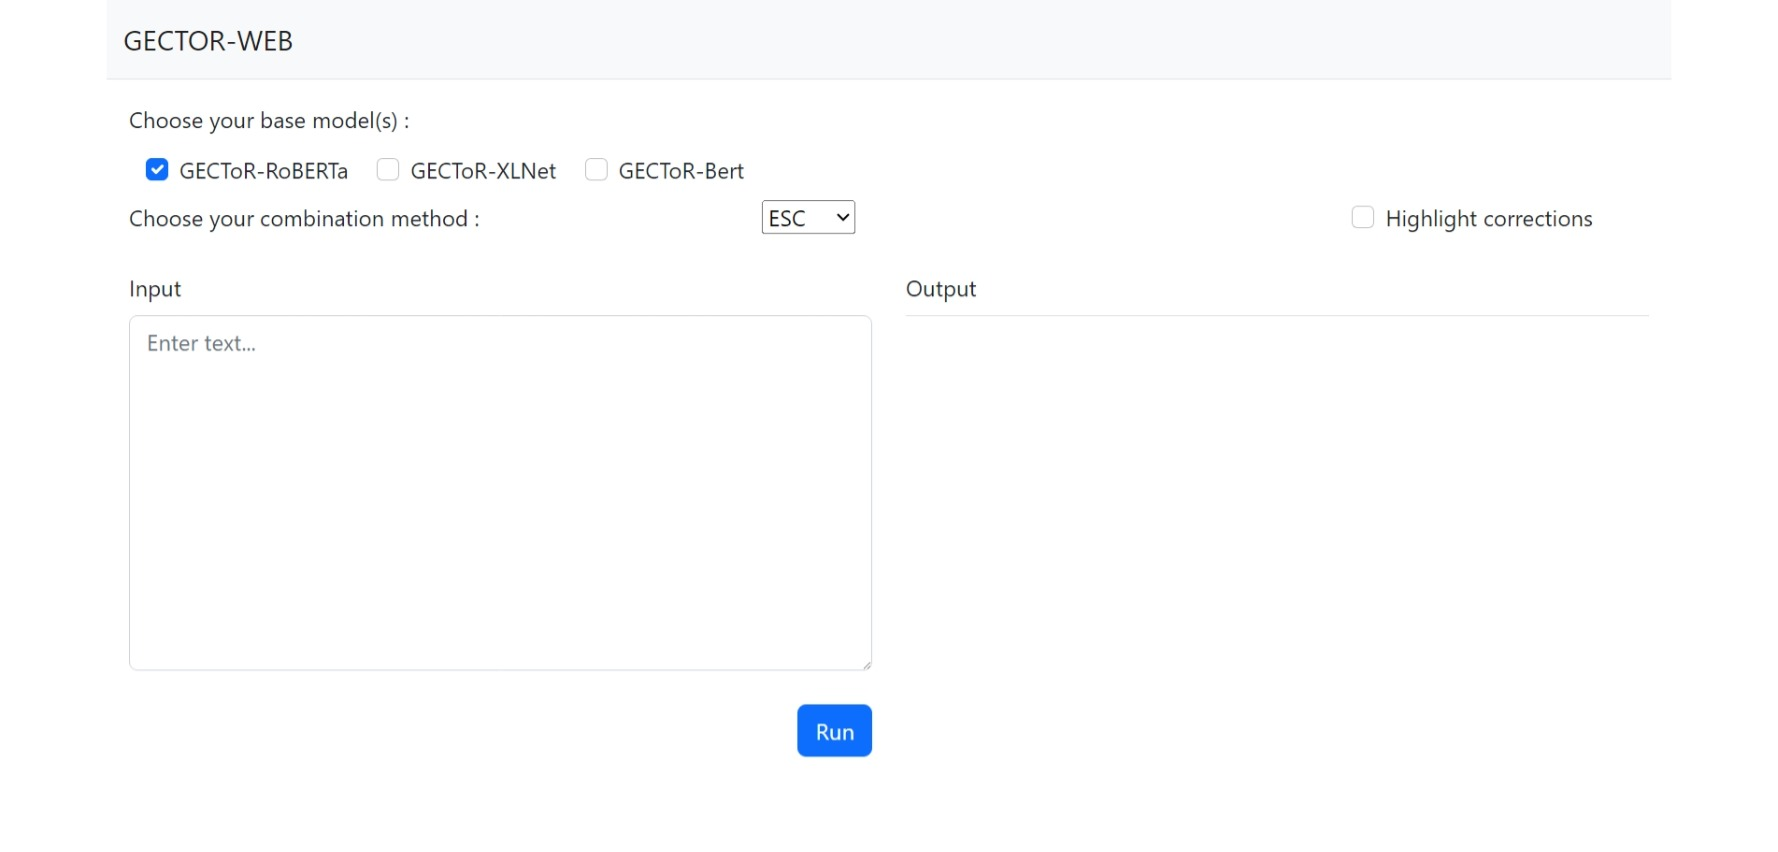
\includegraphics[width=0.85\textwidth]{home}}
      \pause
      \annotatedFigureBox{0.0905,0.7727}{0.4305,0.8393}{i}{0.4305,0.8393}%tr
      \pause
      \annotatedFigureBox{0.434,0.7266}{0.5105,0.8003}{ii}{0.5105,0.8003}%tr
      \pause
      \annotatedFigureBox{0.7615,0.7308}{0.9195,0.7934}{iii}{0.9195,0.7934}%tr
      \pause
      \annotatedFigureBox{0.1285,0.3489}{0.4595,0.6243}{iv}{0.4595,0.6243}%tr
      \pause
      \annotatedFigureBox{0.574,0.2591}{0.8665,0.6118}{v}{0.8665,0.6118}%tr
    \end{annotatedFigure}
    \caption{The User Interface of GecWeb.}
  \end{figure}

  \note<1>{
    The interface of GecWeb consists of five components.
  }

  \note<2>{
    First is the base model selection.

    If the user chooses more than one base model, GecWeb will run a system combination method based on the combination method selected.
  }

  \note<3>{
    Next is the combination method selection.
    If the user only chooses one base system, the selected combination method is ignored.
  }

  \note<4>{
    Thirdly, the user can choose to highlight the corrections by selecting the ``Highlight corrections'' box to, as the name suggests, highlight the corrections in the output text.

    Additionally, it will display simple a explanations to help language learners understand their mistakes better.
  }

  \note<5>{
    The user is then put the text they want to correct in the input text box and clicks the run button.
    The corrected text will then be displayed in the output text box.
  }

  \note<6>{
    After a text is entered into the input text box and the ``Run'' button is clicked, the corrected text will appear in the output text box.
  }
\end{frame}

\subsection{GecWeb Demo}

\begin{frame}{GecWeb Demo (Desktop)}
  \begin{figure}
    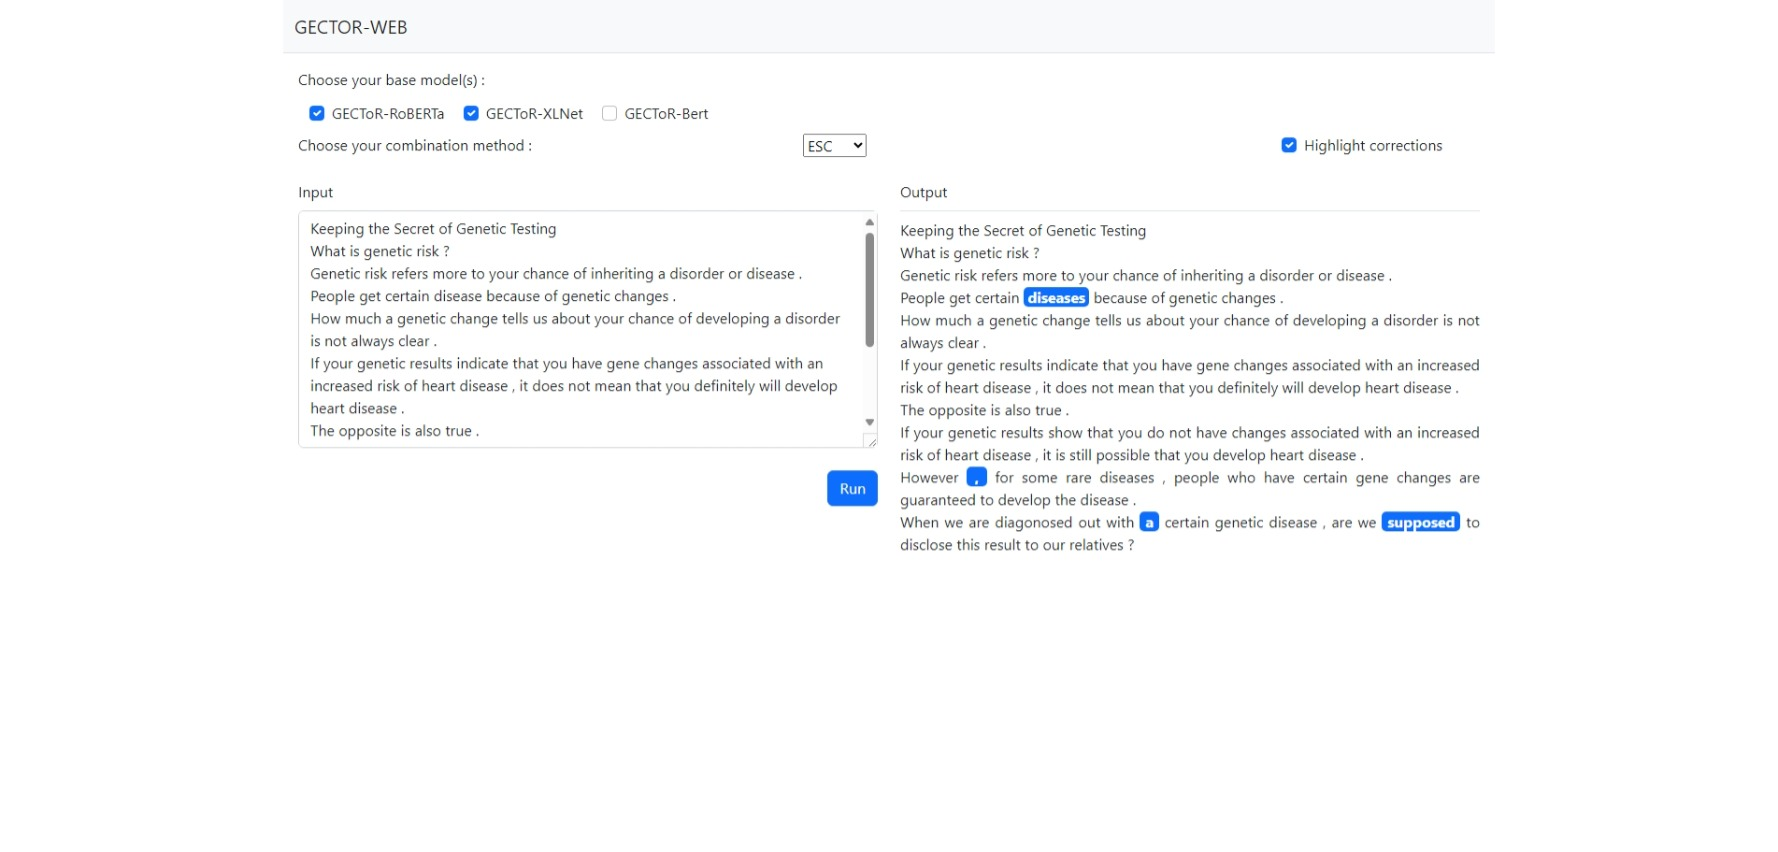
\includegraphics[width=0.9\textwidth]{highlight}
    \caption{GecWeb running on a desktop browser with correction highlights enabled.}
  \end{figure}
\end{frame}

\begin{frame}{GecWeb Demo (Desktop)}
  \begin{figure}
    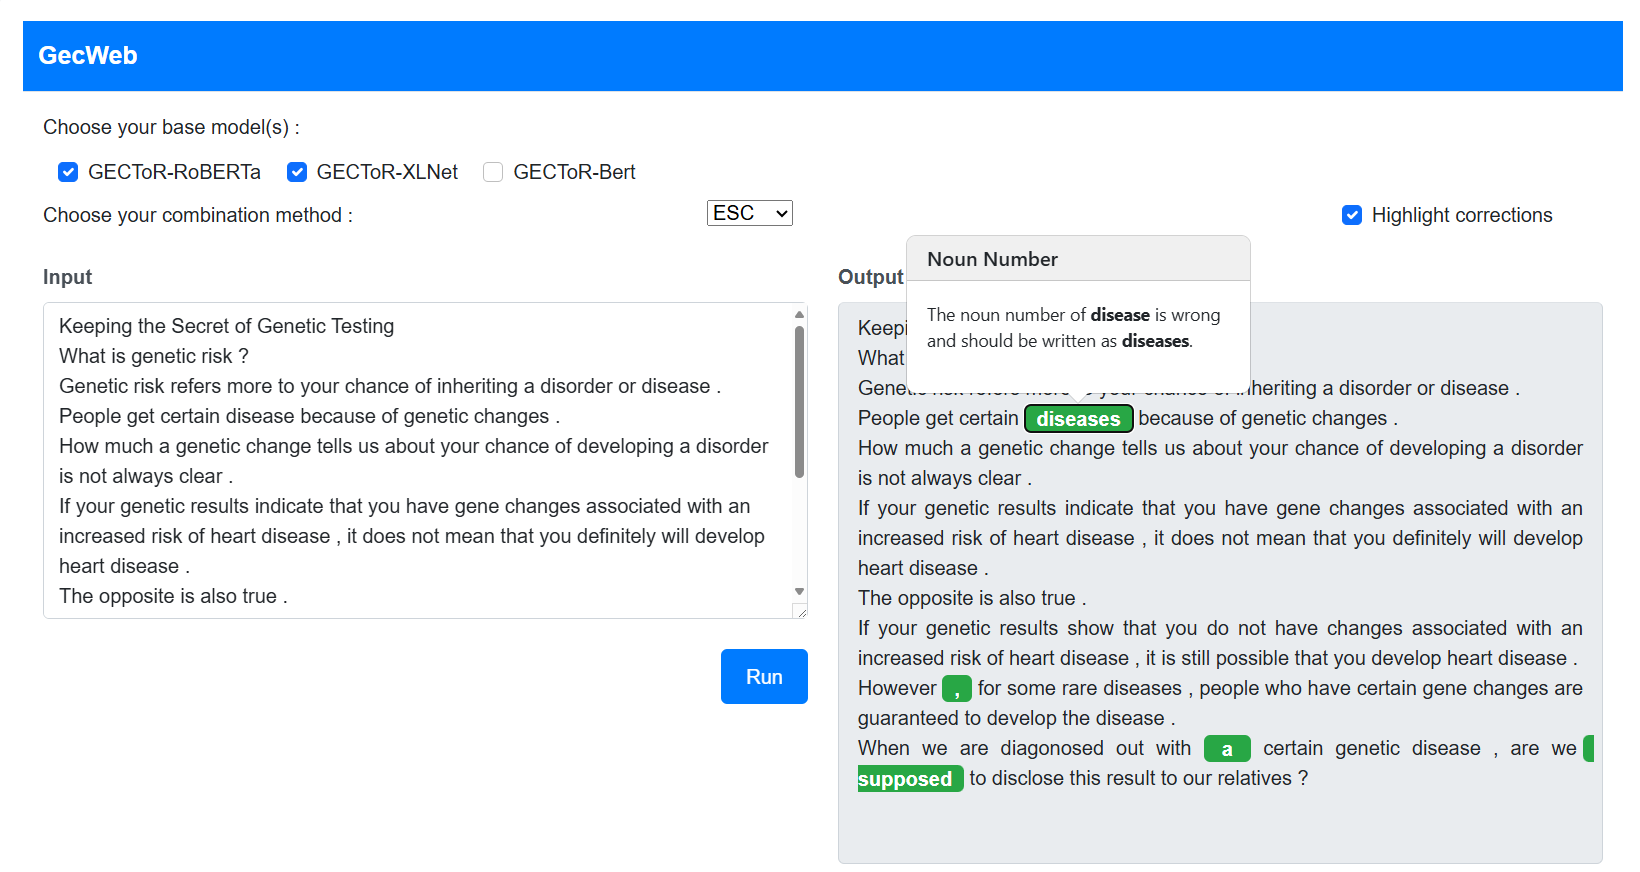
\includegraphics[width=0.8\textwidth]{highlight+note}
    \caption{GecWeb running on a desktop browser with notes about the corrections.}
  \end{figure}
\end{frame}

\begin{frame}{GecWeb Demo (Mobile)}
  \begin{figure}
    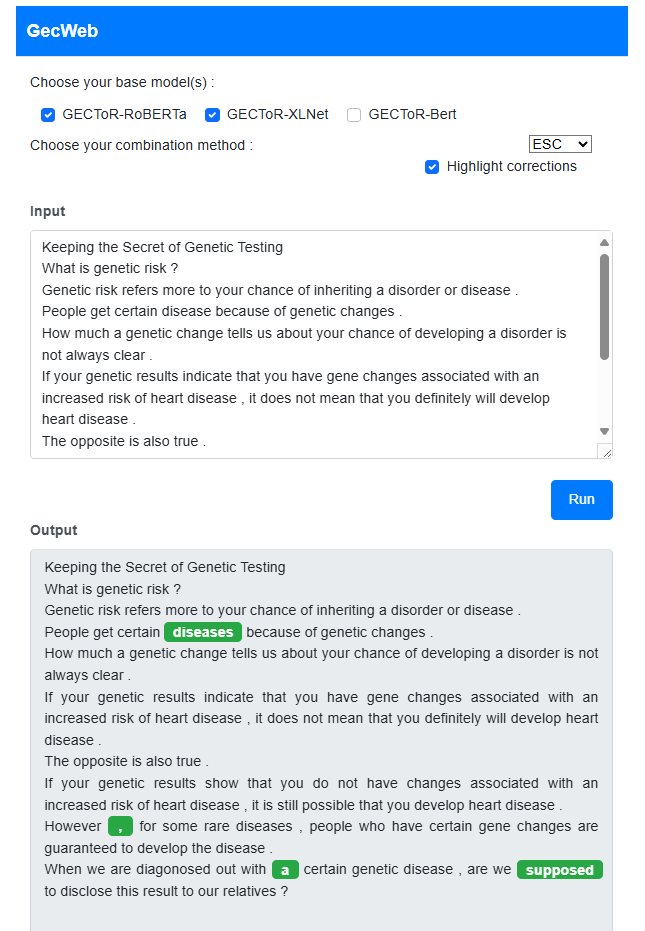
\includegraphics[height=0.75\textheight]{mobile}
    \caption{GecWeb running on a mobile phone.}
  \end{figure}
\end{frame}

\section{Conclusion}


\begin{frame}{References}
  % \nocite{*} % Show all references in the cite.bib file even if they are not cited
  \bibliographystyle{plain}
  \bibliography{cite}
\end{frame}

\begin{frame}{~}
  \begin{center}
    \Large \color{hustred}{Thank you for your attention!}
  \end{center}
\end{frame}

\end{document}
